\section{Rotation of Atomic Orbitals in Space Fixed Axes}
This text should document the implementation of translating and rotating molecular orbitals in
\textsc{Serenity}. The task at hand is to copy a set of molecular orbitals of one molecule and paste
it to an identical molecule that is rotated and translated in space with respect to the original
one.

The main difficulty is to rotate the basis functions used for expanding the molecular orbitals in space,
since it is not strait forward to rotate real spherical harmonics and express the result in the original
basis. Rotation matrices for $s$ and $p$ type functions are trivially, however,
for $d$ or $f$-type functions this is not intuitive any more.

We will start with explaining the construction of the transformation matrices for real spherical harmonics
before describing how this is used to ``copy and paste'' molecular orbitals.

\subsection{Rotation Matrices for Real Spherical Harmonics}

Let us consider two right handed coordinate frames: (i) the Cartesian-coordinate frame in which all basis
functions are expressed in and (ii) the internal-coordinate frame of the molecule. The Cartesian-coordinate
frame may be transformed to the internal-coordinate frame via successive rotations around the $z$ and $y$
axes as
\begin{align}
  \hat{R} = \hat{R}_z(\gamma)\hat{R}_y(\beta)\hat{R}_z(\alpha),
\end{align}
where $\hat{R}_a(\delta)$ is a rotation around axis $a$ by an angle $\delta$. The so-called Euler angles $\alpha$, $\beta$ and $\gamma$ are defined in Fig.~\ref{fig:EulerAnglesDefinition}.

\begin{figure}
  \centering
  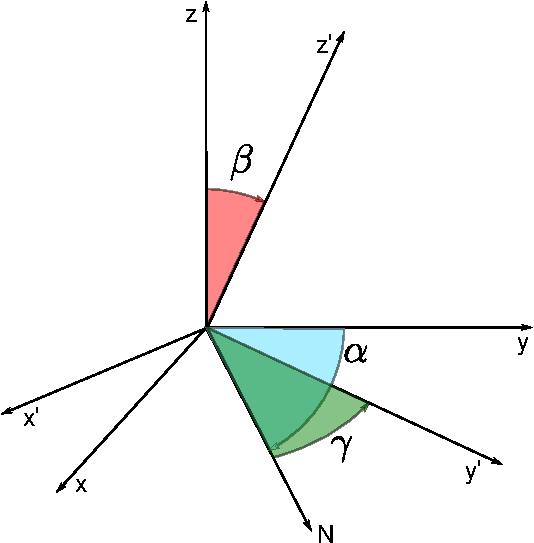
\includegraphics[width = 0.5\textwidth]{figs/eulerAnglesDefinition.pdf}
  \caption{Definition of the Euler angles $\alpha,\beta$ and $\gamma$ used to transform from the coordinate
           frame spanned by $x,y,z$ to the frame spanned by $x^\prime,y^\prime,z^\prime$. The intersection
           between $xy$- and $x^\prime y^\prime $-plane is denoted by $N$. Note that the sign of all angles
           are defined via the plane they are located in ($xy$- or $zy$-plane).}
  \label{fig:EulerAnglesDefinition}
\end{figure}

Molecular orbitals are expressed in terms of so-called real-spherical harmonics $S_{lm}$ (angular momentum $l$
and orientation $m$) which are linear combinations of their complex counter parts $Y_{lm}$, the eigenfunctions
of the angular momentum operator in $z$ direction $\hat{l}_z$. Since the $Y_{lm}$ are degenerate in $m$ for a
radial symmetric Hamiltonian, we are free to construct the linear combinations $S_{lm}$ without changing their
eigenvalue with respect to the Hamiltonian. Thus, the set of functions $S_{lm}$ may be constructed from the
functions $Y_{lm}$ and it may be shown that they represent a complete basis set for a given $l$\cite{Blanco1997}.

The rotation around the $z$-axis may be expressed in terms of the complex-spherical harmonics. In this basis
the rotation matrix associated to $\hat{R}_z$ is diagonal. Thus, the rotation around the $z$ axis may be
expressed in the basis of the real spherical harmonics as
\begin{align}
  \pmb{X}_l(\alpha) = \pmb{C}_l^\dagger \mathrm{Diag}(e^{im\alpha,m=-l,...l})\pmb{C}_l,
\end{align}
where $\mathrm{Diag}(e^{im\alpha,m=-l,...l})$ is the rotation matrix in basis of the complex-spherical harmonics,
and $\pmb{C}_l$ is the (unitary) transformation matrix between real and complex-spherical harmonics.

The matrix representation $\pmb{\Delta}_l(\alpha,\beta,\gamma)$ of the rotation of a set of functions expressed in
the basis of $S_{lm}$ by $\hat{R}$ is then given as
\begin{align}
  \pmb{\Delta}_l(\alpha,\beta,\gamma) = \pmb{X}_l(\alpha) \pmb{D}_l(\beta) \pmb{X}_l(\gamma).
  \label{eq:GeneralRotationWigner}
\end{align}
Here, $\pmb{D}_l(\beta)$ denotes the matrix of the rotation $\hat{R}_y(\beta)$ in the basis of $S_{lm}$
\cite{Blanco1997}.

In 2007 Pinchon and Hoggan\cite{Pinchon2007}, showed that $\pmb{D}_l(\beta)$ may be obtained by first exchanging the
coordinates of $y$ and $z$, rotating around $z$ and then exchanging the coordinates again. If we denote the matrix
for the exchange of $y$ and $z$ in the basis of $S_{lm}$ as $\pmb{J}_l$, we may write
\begin{align}
  \pmb{D}_l(\beta) = \pmb{J}_l \pmb{X}_l(\beta) \pmb{J}_l.
\end{align}
With this, Eq.~(\ref{eq:GeneralRotationWigner}) becomes
\begin{align}
  \pmb{\Delta}_l(\alpha,\beta,\gamma) = \pmb{X}_l(\alpha) \pmb{J}_l \pmb{X}_l(\beta) \pmb{J}_l \pmb{X}_l(\gamma).
  \label{eq:SphericalHarmonicsRotation}
\end{align}
In contrast to previous works\cite{Ivanic1996,Blanco1997}, only the exchange matrices
$\pmb{J}_l$ have to be calculated using recursive schemes, since an explicit expression for the matrix
$\pmb{X}_l(\alpha)$ is known.
It has only non-zero elements on its diagonal and anti-diagonal. For $l=2$, $\pmb{X}_2(\alpha)$ is given by
\begin{align}
  \pmb{X}_2(\alpha) = \begin{pmatrix}
                      \cos(2\alpha) & 0            & 0 & 0            & \sin(2\alpha) \\
                      0             & \cos(\alpha) & 0 & \sin(\alpha) & 0 \\
                      0             & 0            & 1 & 0            & 0 \\
                      0             & -\sin(\alpha)& 0 & \cos(\alpha) & 0 \\
                      -\sin(2\alpha)& 0            & 0 & 0            & \cos(2\alpha)
                      \end{pmatrix}.
\end{align}

The recurrence expressions for $\pmb{J}_l$ for $l \leq 1$ are given by
\begin{align}
  \begin{split}
    \pmb{G}^l_x \pmb{J}_l &= \pmb{J}_{l+1}\pmb{G}^l_x\\
    \pmb{G}^l_z \pmb{J}_l &= \pmb{J}_{l+1}\pmb{G}^l_y\\
    \pmb{G}^l_y \pmb{J}_l &= \pmb{J}_{l+1}\pmb{G}^l_z,
  \end{split}
  \label{eq:GauntTransformation}
\end{align}
where $\pmb{G}^l_x$, $\pmb{G}^l_y$ and $\pmb{G}^l_z$ are the matrices of the so-called Gaunt coefficients. Their
non-zero elements are given by
\begin{align}
  \begin{split}
    \kappa_l &= \frac{1}{2\sqrt{(2l+1)(2l+3)}},\\
    \left(\pmb{G}^l_x\right)_{2+k,k} = \left(\pmb{G}^l_x\right)_{2l+2-k,2l+2-k}&
    = \left(\pmb{G}^l_y\right)_{2l+2-k,k} = -\left(\pmb{G}^l_y\right)_{2+k,2l+2-k}\\
    &= \kappa_l\sqrt{k(k+1)},
    ~~~1\leq k \leq l-1,\\
    \left(\pmb{G}^l_x\right)_{k,k} = \left(\pmb{G}^l_x\right)_{2l+4-k,2l+2-k}
    &= \left(\pmb{G}^l_y\right)_{k,2l+2-k} = -\left(\pmb{G}^l_y\right)_{2l+4-k,k}\\
    &=-\kappa_l \sqrt{(2l+2-k)(2l+3-k},
    ~~~1\leq k \leq l,\\
    \left(\pmb{G}^l_x\right)_{l+2,l+2} = \left(\pmb{G}^l_y\right)_{l+2,l} &= \kappa_l \sqrt{2l(l+1)},\\
    \left(\pmb{G}^l_x\right)_{l+3,l+1} = \left(\pmb{G}^l_y\right)_{l+1,l+1} &= -\kappa_l \sqrt{2(l+1)(l+2)},\\
    \left(\pmb{G}^l_z\right)_{k+1,k} &= 2\kappa_l \sqrt{k(2l+2-k)},~~~ 1 \leq k \leq 2l+1.
  \end{split}
\end{align}
In order to calculate the entries of $\pmb{J}_l$, only the diagonal, non-zero block ($\hat{\pmb{G}}^l_z$)
of $\pmb{G}^l_z$ and $\pmb{G}^l_y$ are needed. $\pmb{J}_{l+1}$ may then be written as
\begin{align}
  \pmb{J}_{l+1} = \begin{pmatrix}
                    0      & ~ & 0 \\
                    \vdots &  \pmb{G}^l_y \pmb{J}_{l} \left(\hat{\pmb{G}}^l_z\right)^{-1} & \vdots\\
                    0      & ~ & 2^{-l}
                  \end{pmatrix},
  \label{eq:Recurrence}
\end{align}
where the central block of columns (all columns except the first and last one) are given by
$\pmb{G}^l_y \pmb{J}_{l} \left(\hat{\pmb{G}}^l_z\right)^{-1}$. The missing rows of the first and last column
can be constructed from the requirement of the matrix $\pmb{J}_{l}$ to be symmetric.

The matrices $\pmb{J}_{l}$ for $l=1$ and $l=0$ are given by
\begin{align}
  \pmb{J}_{0} = \begin{pmatrix}
                    1
                  \end{pmatrix},
\end{align}
and
\begin{align}
  \pmb{J}_{1} = \begin{pmatrix}
                  0 & -1 & 0 \\
                  -1&  0 & 0 \\
                  0 &  0 & 1
                \end{pmatrix}.
\end{align}
All other matrices for $l > 1$ may be computed using Eq.~(\ref{eq:Recurrence}).

\subsection{Copying and Pasting Molecular Orbitals}

Consider two molecules $A$ and $B$ which are identical up to translation and rotation. The molecular-orbitals set
$\{\psi^{A}_i\}$ of molecule $A$ is known and expressed in a set of spherical, atom-centered basis functions with
coefficients $\pmb{C}^A$. Our goal is to obtain the coefficients $\pmb{C}^B$ that correspond to the set
$\{\psi^{B}_i\}$ by translating and rotating the set $\{\psi^{A}_i\}$. Since the atoms of both molecules are the same,
their exists a one to one mapping of basis function shells. Thus, the translational part is trivially taken care of,
i.e. if the molecules are not rotated with respect to each other the coefficient matrices $\pmb{C}^A$ and
$\pmb{C}^B$ will be identical. In case of rotation, we first calculate the Euler angles ($\alpha_A$, $\beta_A$,
$\gamma_A$) for the rotation of the Cartesian frame to the internal frame of $A$. We can then rotate the
$\{\psi^{A}_i\}$ to the Cartesian frame by rotating the coefficient matrix in a shell-wise manner with the
transformation matrix $\pmb{\Delta}_l$ from Eq.~(\ref{eq:SphericalHarmonicsRotation}),
\begin{align}
  \left(\pmb{C}^\mathrm{Cart}\right)_{\mu_l} = \pmb{\Delta}_l(-\gamma_A,-\beta_A,-\alpha_A)\left(\pmb{C}^A\right)_{\mu_l},
\end{align}
where the subscript ${\mu_l}$ denotes the basis-function block associated to the shell $\mu_l$ with
angular momentum $l$.

The orbitals can then be rotated from the Cartesian frame to the internal frame of $B$ with the Euler angles
for the rotation of the Cartesian to the internal frame $B$ ($\alpha_B$, $\beta_B$, $\gamma_B$) as
\begin{align}
  \left(\pmb{C}^B\right)_{\mu_l} = \pmb{\Delta}_l(\alpha_B,\beta_B,\gamma_B)\left(\pmb{C}^\mathrm{Cart}\right)_{\mu_l}.
\end{align}

\subsection{Internal Frame Construction}

Each molecule is represented by the coordinates of its atoms $\{\pmb{a}_i\}$ in the Cartesian frame.
The internal $x$-axis $\pmb{e}_x$ is constructed as
\begin{align}
  \pmb{e}_x = \frac{(\pmb{a}_1-\pmb{a}_0)}{|\pmb{a}_1-\pmb{a}_0|},
\end{align}
the $y$-axis is constructed as
\begin{align}
  \pmb{e}_y = \frac{\pmb{t}_y}{|\pmb{t}_y|},
\end{align}
where $\pmb{t}_y$ is the orthogonalized difference vector between the coordinates of $1$ and $2$
which is defined with the difference vector $\pmb{d}_{21} = \pmb{a}_2-\pmb{a}_1$ as
\begin{align}
  \pmb{t}_y = \pmb{d}_{21}-\pmb{e}_x\pmb{e}_x^\dagger\pmb{d}_{21}.
\end{align}
The $z$-axis that belongs to a right-handed coordinate system can then be obtained as
\begin{align}
  \pmb{e}_z = \pmb{e}_x \times \pmb{e}_y.
\end{align}
Note that some special cases for highly symmetrical molecules need to be handled:
(i)   If the molecule consists of only one atom, the Cartesian frame is used as the internal frame.
(ii)  If the molecule consists of only two atoms, the vector $\pmb{d}_{21}$ is chosen to be the Cartesian
      $x$-axis if $\pmb{e}_x$ does not depend linearly on it. Otherwise the $y$-axis is chosen.
(iii) If the vector $\pmb{d}_{21}$ is linear depended on $\pmb{e}_x$, the difference vector $\pmb{d}_{31}$ is
      chosen for the construction of $\pmb{e}_y$. This is repeated until $\pmb{e}_y$ can be constructed. If there
      is no linear independent difference vector, the approach given in (ii) is used.
